% This is samplepaper.tex, a sample chapter demonstrating the
% LLNCS macro package for Springer Computer Science proceedings;
% Version 2.20 of 2017/10/04
%
\documentclass[runningheads]{llncs}
%
%%%%%ДОБАВИЛ ДЛЯ РУССКОГО ТЕКСТА
\usepackage[utf8x]{inputenc}
\usepackage[english,russian]{babel}
\usepackage{cmap}
%%%%%
\usepackage{eqnarray,amsmath}
\usepackage{subfig}
\usepackage{graphicx}
\usepackage{amsfonts}
\usepackage{amssymb}
% Used for displaying a sample figure. If possible, figure files should
% be included in EPS format.
%
% If you use the hyperref package, please uncomment the following line
% to display URLs in blue roman font according to Springer's eBook style:
% \renewcommand\UrlFont{\color{blue}\rmfamily}
\setlength{\textfloatsep}{4pt plus 1.0pt minus 1.5pt}
\setlength{\floatsep}{4pt plus 1.0pt minus 1.5pt}
%\setlength{\abovedisplayskip}{3pt}
%\setlength{\belowdisplayskip}{3pt}

\begin{document}
%
\title{Comparison of dimensionality reduction schemes for parallel global optimization algorithms
\thanks{The study was supported by the Russian Science Foundation, project No 16-11-10150}}
%
%\titlerunning{Abbreviated paper title}
% If the paper title is too long for the running head, you can set
% an abbreviated paper title here
%
\author{Konstantin Barkalov \and
Vladislav Sovrasov \and
Ilya Lebedev}
%
\authorrunning{K. Barkalov et al.}
% First names are abbreviated in the running head.
% If there are more than two authors, 'et al.' is used.
%
\institute{
Lobachevsky State University of Nizhny Novgorod, Nizhny Novgorod, Russia
\email{konstantin.barkalov@itmm.unn.ru}\\
\email{sovrasov.vlad@gmail.com}\\
\email{ilya.lebedev@itmm.unn.ru}\\
\url{http://hpc-education.unn.ru/основные-напраления/глобальная-оптимизация} }
%
\maketitle              % typeset the header of the contribution
%
\begin{abstract}
This work considers a parallel algorithms for solving multi-extremal optimization problems. Algorithms are developed within the framework of the information-statistical approach and implemented in a parallel solver “Globalizer” . The optimization problem is solved by reducing the multidimensional problem to a set of joint one-dimensional problems that are solved in parallel. Five types of Peano-type space-filling curves are employed to reduce dimension. The results of computational experiments carried out on several hundred test problems are discussed.

\keywords{Global optimization \and  Dimension reduction \and Parallel algorithms  \and Multidimensional multiextremal optimization  \and Global search algorithms  \and Parallel computations }
\end{abstract}

%------------------------------------------------------------------------------
\section{Introduction}\label{sec:intro}


%------------------------------------------------------------------------------
\section{Statement of Multidimensional Global Optimization Problem}
In this paper, the core class of optimization problems, which can be solved using
Globalizer\cite{globalizerSystem}, is formulated. This class involves the multidimensional global
optimization problems without constraints, which can be defined in the following way:
\begin{equation}
\label{eq:task}
\begin{array}{cr}\\
  \varphi(y^*)=\min\{\varphi(y):y\in D\}, \\
  D=\{y\in \mathbb{R}^N:a_i\leq y_i\leq{b_i}, 1\leq{i}\leq{N}\}
\end{array}
\end{equation}
with the given boundary vectors  $a$ and  $b$. It is supposed, that the objective function \(\varphi(y)\) satisfies the Lipschitz condition
\begin{equation}
\label{eq:lip}
|\varphi(y_1)-\varphi(y_2)|\leq L\Vert y_1-y_2\Vert,y_1,y_2\in D,
\end{equation}
where \(L>0\) is the Lipschitz constant, and \(||\cdot||\) denotes the norm in \(\mathbf{R}^N\) space.
\par
Usually, the minimized function \(\varphi(y)\) is defined as a computational procedure,
according to which the value \(\varphi(y)\) can be calculated for any vector \(y\in D\)
(let us further call such a calculation \textit{a trial}). It is supposed that this procedure
is a time-consuming one. As a result, the overall time of solving the optimization
problem (\ref{eq:task}) is determined, first of all by the number of executed trials.
It should also be noted that the requirement of the Lipschitz condition (\ref{eq:lip})
is highly important, since an estimate of the global minimum can be constructed on the
basis of a finite number of computed values of the optimized function only in this case .

%------------------------------------------------------------------------------
\section{Methods of Dimension Reduction}
\subsection{Single evolvent}

Within the framework of the information-statistical global optimization theory,
the Peano space-filling curves (or evolvents) \(y(x)\) mapping the interval \([0,1]\)
onto an \(N\)-dimensional hypercube \(D\) unambiguously are used for the dimensionality
reduction \cite{sergeyevStronginLera2013}, \cite{strongin1978}, \cite{stronginGergelBarkalovParGO}, \cite{strSergGO}.
\par
As a result of the reduction, the initial multidimensional global optimization
problem (\ref{eq:task}) is reduced to the following one-dimensional problem:
\begin{equation}
\label{eq:oneDimTask}
\varphi(y(x^*))=\min\{\varphi(y(x)):x\in [0,1]\}.
\end{equation}
\par
It is important to note that this dimensionality reduction scheme transforms the minimized
Lipschitzian function from (\ref{eq:task}) to the corresponding one-dimensional
function \(\varphi(y(x))\), which satisfies the uniform H{\"o}lder condition, i. e.
\begin{equation}
\label{eq:holder}
|\varphi(y(x_1))-\varphi(y(x_2))|\leq H{|x_1-x_2|}^{\frac{1}{N}}, x_1,x_2\in[0,1],
\end{equation}
where the constant $H$ is defined by the relation \(H=2L\sqrt{N+3}\), \(L\) is the Lipschitz
constant from (\ref{eq:lip}), and \(N\) is the dimensionality of the optimization problem (\ref{eq:task}).
\par
The algorithms for the numerical construction of the Peano curve approximations are
given in \cite{strSergGO}.

\par
The computational scheme obtained as a result of the dimensionality reduction consists of the following:
\begin{itemize}
  \item The optimization algorithm performs the minimization of the reduced one-dimensional
  function \(\varphi(y(x))\) from (\ref{eq:oneDimTask}),
  \item After determining the next trial point \(x\), a multidimensional image \(y\) is calculated by using the
mapping \(y(x)\),
  \item The value of the initial multidimensional function \(\varphi(y)\) is calculated at the point \(y\in D\),
  \item The calculated value \(z=\varphi(y)\) is used further as the value of the reduced one-dimensional function \(\varphi(y(x))\) at the point \(x\).
\end{itemize}

%------------------------------------------------------------------------------
\subsection{Shifted evolvents}
\label{sec:shifted}

The reduction of the multidimensional problems to the one-dimensional ones using the Peano curves has such important properties as the continuity and the uniform boundedness of the function differences for limited variation of argument. However, a partial loss of information on the nearness of the points in the multidimensional space takes place since a point $x \in [0,1]$ has the left and the right neighbors only while the corresponding point $y(x) \in D \subset R^N$ has the neighbors in $2N$ directions. As a result, when using the mappings like Peano curve the images $y',\ y'',$ which are close to each other in the $N$-dimensional space can correspond to the preimages $x',\ x'',$ which can be far away from each other in the interval $[0,1]$. This property results in the excess computations since several limit points $x',\ x''$ of the trial sequence generated by the index method in the interval $[0,1]$ can correspond to a single limit point $y$ in the $N$-dimensional space.

One of the possible ways to overcome this disadvantage consists in using the multiple mappings
\begin{equation}%\label{eq:142}
Y_L(x)=\left\{y^0(x),\ y^1(x),...,\ y^L(x)\right\}
\end{equation}
instead of single Peano curve $y(x)$ (see \cite{Strongin1991,Strongin1992,strSergGO}).

Such set of evolvents can be produced by shifting the source evolvent $y^0(x)$ by $2^{-l},0 \leq l \leq L$ on each coordinate. Each evolvent has it's own corresponding hypercude $D_l= \left\{y \in R^N: -2^{-1} \leq y_i+2^{-l} \leq 3 \cdot 2^{-1},\ 1\leq i\leq N\right\},\ 0 \leq l \leq L$.

In Fig.~\ref{fig:shifted_ev} the image of the interval $[0,1]$ obtained by the curve $y^0(x),\ x\in [0,1],$ is shown as the dashed line. Since the hypercube $D$ from (\ref{eq:task}) is included in the common part of the family of hypercubes $D_l$ (the boundaries of hypercube $D$ are highlighted in Fig.~\ref{fig:shifted_cube}), having introduced an additional constraint function
\begin{equation}\label{6_g0}
g_0(y)=\max\left\{\left|y_i\right| - 2^{-1}:\ 1\leq i\leq N\right\},
\end{equation}
one can present the initial hypercube $D$ in the form
\[
D=\left\{y^l(x):\; x\in [0,1],\ g_0(y^l(x))\leq 0 \right\},\ 0\leq l \leq L,
\]
i.e., $g_0(y) \leq 0$ if $y\in D$ and $g_0(y)>0$ otherwise. Consequently, any point $y \in D$ has its own preimage $x^l \in [0,1]$ for each mapping $y^l(x),\ 0\leq l\leq L$.

Thus, each evolvent $y^l(x),\ 0\leq l \leq L,$ generates its own problem of the type (\ref{eq:task}) featured by its own extended (in comparison with $D$) search domain $D_l$ and the additional constraint with the left hand part from (\ref{6_g0})
\begin{equation}\label{6_problem_l}
\min{\left\{\varphi(y^l(x)):x\in [0,1], \; g_j(y^l(x))\leq 0, \; 0 \leq j \leq m\right\}}, \ 0 \leq l \leq L.
\end{equation}

\begin{figure}[ht]
    \centering
    \subfloat[Two mappings]{{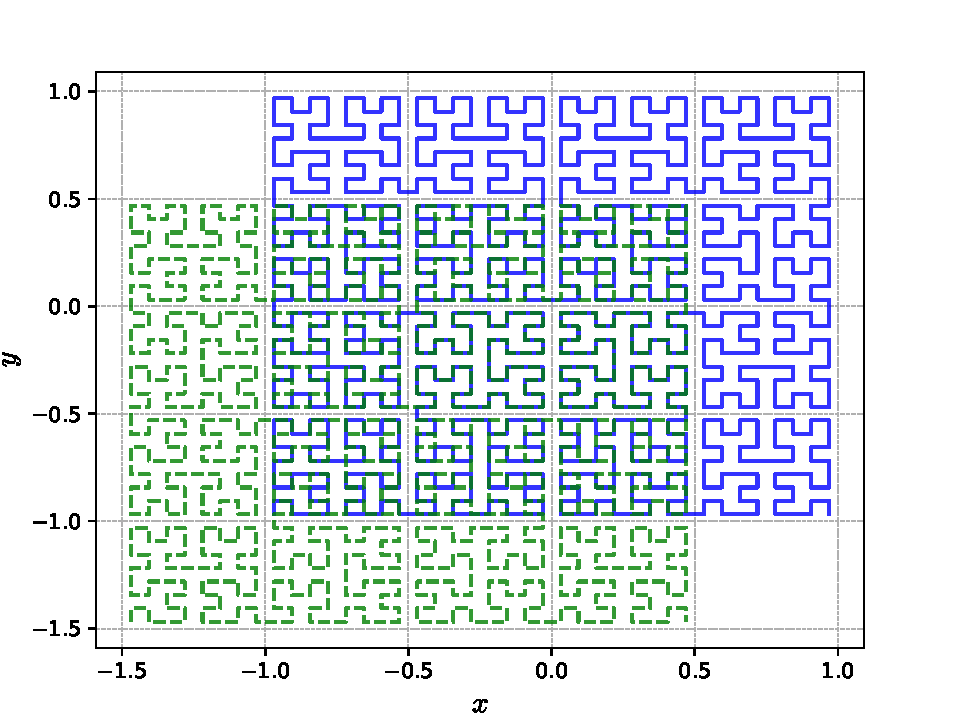
\includegraphics[width=.6\textwidth]{pictures/shifted.pdf}}\label{fig:shifted_ev}}
    \subfloat[Hypercubes $D_l$]{{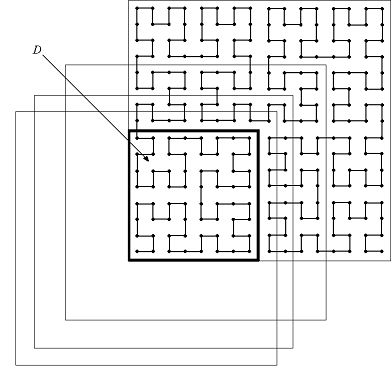
\includegraphics[width=.4\textwidth]{pictures/shifted_cube.png}}\label{fig:shifted_cube}}
    \caption{Multiple mappings}
\end{figure}

%------------------------------------------------------------------------------
\subsection{Rotated evolvents}
The application of the scheme for building the multiple evolvents (hereinafter called the shifted evolvents or $S$-evolvents) described in Subsection \ref{sec:shifted} allows to preserve the information on the nearness of the points in the multidimensional space and, therefore, to provide more precise (as compared to a single evolvent) estimate of Lipschitz constant in the search process. However, this approach has serious restrictions, which narrow the applicability of the parallel algorithms, designed on the base of the $S$-evolvents (see te end of the section \ref{sec:seq_comp}).

To overcome the $S$-evolvent and to preserve the information on the nearness of the points in the $N$-dimensional space, a novel scheme of building of the multiple mappings is proposed. The building of a set of Peano curves not by the shift along the main diagonal of the hypercube but by rotation of the evolvents around the coordinate origin is a distinctive feature of the proposed scheme \cite{Gergel2009}. In the initial non-rotated mapping for close points $y', y''$ in the multidimensional space their preimages  $x', x''$ in the interval $[0,1]$ can be far away from each other. In the rotated scheme there exists a mapping $y^i(x)$ according to which preimages $x', x''$ will be located nearer. The evolvents generated according to this scheme are called the rotated evolvents or $R$-evolvents.

In Fig.~\ref{6_fig_9} two evolvents being the approximations to Peano curves for the case $N=2$ are presented as an illustration.
Taking into account the initial mapping, one can conclude that current implementation of the method allows to build up to $N(N-1)+1$ evolvents for mapping the $N$-dimensional domain onto the corresponding one-dimensional intervals. Moreover, the additional constraint  $g_0(y) \leq 0$ with $g_0(y)$ from (\ref{6_g0}), which arises in shifted evolvents, is absent. This method for building a set of mappings can be ``scaled'' easily to obtain more evolvents (up to $2^N$) if necessary.

\begin{figure}[t]
  \centering
  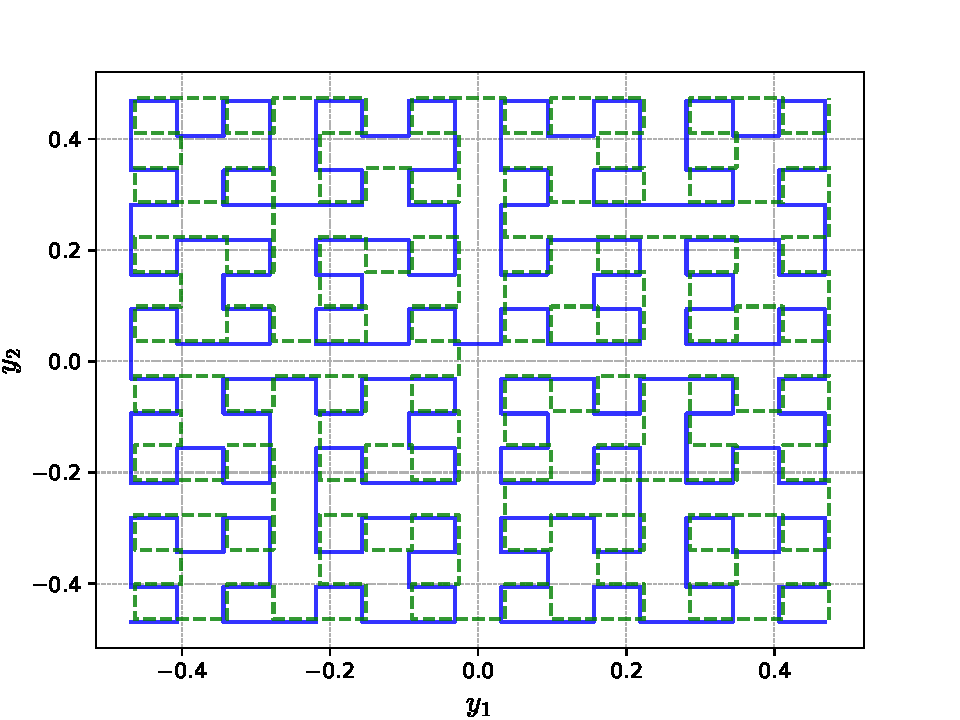
\includegraphics[width=0.6\linewidth]{pictures/rotated_1.pdf}
  \caption{Two rotated evolvents on the same plane}
  \label{6_fig_9}
\end{figure}

%------------------------------------------------------------------------------
\subsection{Non injective evolvent}

Как уже было сказано в секции \ref{sec:shifted}, потеря информации о близости точек в многомерном пространстве может быть частично скомпенсирована использованием множественных отображений $Y_L(x)=\{y^1(x),...,y^L(x)\}$. Однако, сама по себе кривая типа Пеано сохраняет в себе часть этой информации: она не является инъективым отображением, поэтому имея один образ $y(x)\in \mathbb{R}^N$, можно получить несколько несколько отличных $x$ прообразов $t_j\in[0,1], t_j \not = x$, которые затем могут быть добавлены в поисковую информацию индексного метода.

Кривая типа Пеано, используемая в (\ref{eq:oneDimTask}) для редукции размерности, определяется через предельный переход,
поэтому не может быть вычислена непосредтвенно. При численной оптимизации используется некоторое её приближение, являющееся
инъективной кусочно-линейной кривой. В \cite{strongin1978} было предложено неинъективное отображение равномерной сетки на отрезка $[0,1]$ на равномерную сетку в гиперкубе $D$. Каждый многомерный узел может иметь до $2^N$ одномерных прообразов. На рис. \ref{fig:noninjective} изображена кривая с самопересечениями, полученная при соединении узлов грубой многомерной сетки в порядке следования их прообразов из отрезка $[0,1]$, а также отмечана точка, имеющая 3 прообраза.

Недостатком неинъективной развёртки является потенциально большое количетво прообразов (до $2^N$) и невозможность использования параллельной схемы для множественных отображений из секции \ref{sec:parallel_evolvents}.

%------------------------------------------------------------------------------
\subsection{Smooth evolvent}

\begin{figure}[ht]
    \centering
    \subfloat[Smooth evolvent]{{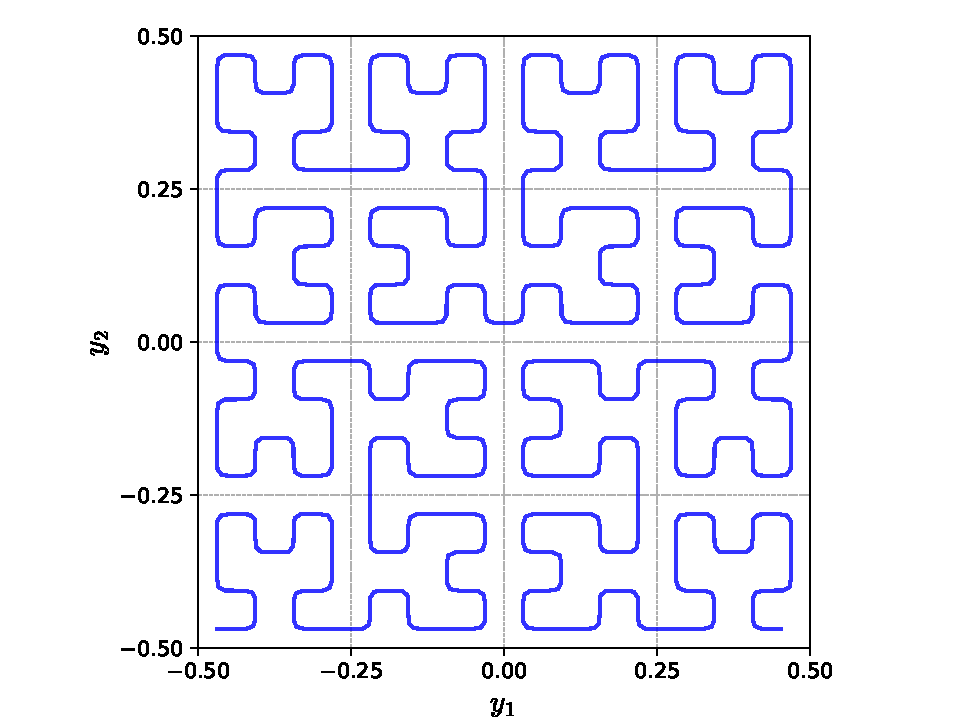
\includegraphics[width=.6\textwidth]{pictures/smooth.pdf}}\label{fig:smooth}}
    \subfloat[Numerical non injective evolvent]{{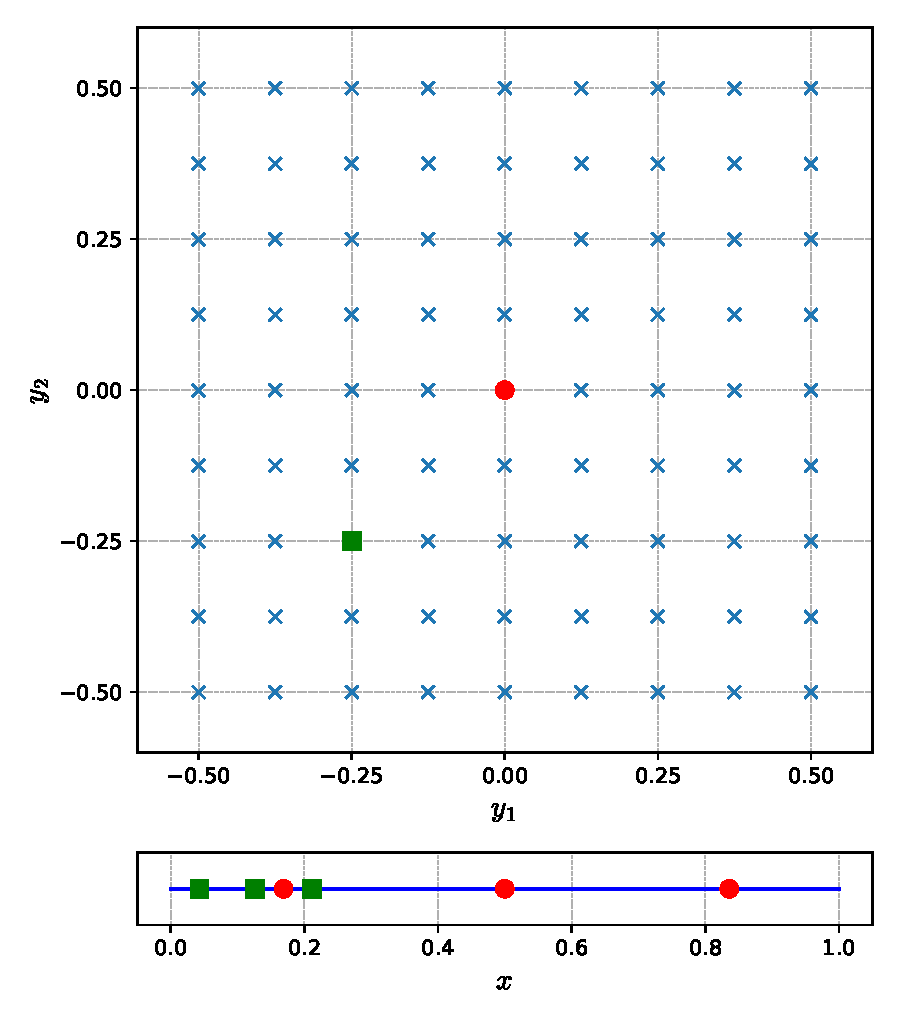
\includegraphics[width=.4\textwidth]{pictures/noninjective.pdf}}\label{fig:noninjective}}
    \caption{Different evolvents}
\end{figure}

\section{Parallel Computations for Solving Global Optimization Problems.}
\subsection{Core Multidimensional Algorithm of Global Search}

The optimization methods applied in Globalizer to solve the reduced problem (\ref{eq:oneDimTask}) are based on the MAGS method, which can be presented as follows --- see \cite{strongin1978}, \cite{strSergGO}.
\par
The initial iteration of the algorithm is performed at an arbitrary point \mbox{\(x^1\in(0,1)\)}.
Then, let us suppose that \(k\), \(k\ge 1\), optimization iterations have been completed already.
The selection of the trial point \(x^{k+1}\) for the next iteration is performed according to the following rules.

\textit{Rule 1}. Renumber the points of the preceding trials by the lower indices in order of increasing value of coordinates
$0=x_0<x_1<...<x_{k+1}=1$.

\textit{Rule 2}. Compute the characteristics \(R(i)\) for each interval \((x_{i-1},x_i),1\leq i\leq k+1\).

\textit{Rule 4}. Determine the interval with the maximum characteristic $R(t)=\max_{1\leq i \leq k+1}R(i)$.

\textit{Rule 5}. Execute a new trial at the point \(x^{k+1}\) located within the interval with the maximum characteristic from the previous step
  $x^{k+1}=d(x_t)$.

The stopping condition, which terminated the trials, is defined by the inequality $\rho_t<\varepsilon$
for the interval with the maximum characteristic from Step 4 and \(\varepsilon >0\) is the predefined
accuracy of the optimization problem solution. If the stopping condition is not satisfied,
the index \(k\) is incremented by 1, and the new global optimization iteration is executed.

The convergence conditions and exact formulas for descision rules $R(i)$ and $d(x)$ of the described algorithm are given, for example, in \cite{strSergGO}.

%------------------------------------------------------------------------------
\subsection{Parallel algorithm exploiting a set of evolvents}
\label{sec:parallel_evolvents}
Using the multiple mapping allows solving initial problem (\ref{eq:task}) by parallel solving the problems
\[
\min\{\varphi(y^s(x)):x\in [0,1]\}, 1\leqslant s\leqslant S
\]
on a set of intervals $[0,1]$ by the index method. Each one-dimensional problem is solved on a separate processor. The trial results at the point \(x^k\) obtained for the problem being solved by particular processor are interpreted as the results of the trials in the rest problems (in the corresponding points \(x^(k_1 ),\dots,x^(k_S))\). In this approach, a trial at the point \(x^k \in [0,1]\) executed in the framework of the \(s\)-th problem, consists in the following sequence of operations.
\par
1. Determine the image \(y^k=y^s (x^k)\) for the evolvent \(y^s (x)\).
\par
2. Inform the rest of processors about the start of the trial execution at the point\( y^k\) (the blocking of the point \(y^k\) ).
\par
3. Determine the preimages \(x{}^{k_s}  \in [0,1], 1≤s≤S\), of the point \(y^k\) and interpret the trial executed at the point \(y^k \in D \) as the execution of the trials in the \(S\) points \(x{}^{k_1} ,…,x{}^{k_s} \)
\par
4. Inform the rest of processors about the trial results at the point \(y^k\).
\par

The decision rules for the proposed parallel algorithm, in general, are the same as the rules of the sequential algorithm (except the method of the trial execution). Each processor has its own copy of the software realizing the computations of the problem functions and the decision rule of the index algorithm. For the organization of the interactions among the processors, the queues are created on each processor, where the processors store the information on the executed iterations in the form of the tuples: the processor number \(s\), the trial point \(x{}^{k_s}\).
\par
The proposed parallelization scheme was implemented with the use of MPI technology. Main features of implementation consist in the following. A separate MPI-process is created for each of \(S\) one-dimensional problems being solved, usually, one process per one processor employed. Each process can use p threads, usually one thread per an accessible core.
\par
At every iteration of the method, the process with the index \(s,0\leqslant s< S\) performs p trials in parallel at the points \(x^{(s+i_S)},0\leqslant i<p\). At that, each process stores all \(S_p\) points, and an attribute indicating whether this point is blocked by another process or not is stored for each point. Let us remind that the point is blocked if the process starts the execution of a trial at this point.
\par
At every iteration of the algorithm, operating within the \(s\)-th process, determines the coordinates of p «its own» trial points. Then, the interchange of the coordinates of images of the trial points \(y^{(s+i_S)},0\leqslant i<p, 0\leqslant s< S\) is performed (from each process to each one). After that, the preimages \(x^{(q+i_S)},0\leqslant q<S,q\not=s\) of the points received by the \(s\)-th process from the neighbor ones are determined with the use of the evolvent \(y^s (x)\). The points blocked within the \(s\)-th process will correspond to the preimages obtained. Then, each process performs the trials at the non-blocked points, the computations are performed in parallel using OpenMP. The results of the executed trials (the index of the point, the computed values of the problem functions, and the attribute of unblocking of this point) are transferred to all rest processes. All the points are added to the search information database, and the transition to the next iteration is performed.
\par

%------------------------------------------------------------------------------
\section{Results of Numerical Experiments}
The computational experiments have been carried out on the Lobachevsky supercomputer at
State University of Nizhny Novgorod. A computational node included 2 Intel
Sandy Bridge E5-2660 2.2 GHz processors, 64 GB RAM. The CPUs had 8 cores (i. e. total 16 cores
were available per a node). Все рассматриваемые алгортимы и развёртки были реализованы на языке C++ в рамках программной системы Globalizer\cite{globalizerSystem}.
Для реализации параллелизма на одном узле использована технология OpenMP, а для параллелизма на несколько узлов --- стандарт MPI.

Сравнение алгоритмов глобальной оптимизации проведено путём оценки качества решения алгоритмами выборки задач из некоторого тестового класса.
В данной статье рассматривается тестовый класс, порождаемый генератором GKLS \cite{Gaviano2003}. Данные генератор позволяет конструировать сложные многоэкстремальные задачи различной размерности. В работе рассматриваются выборки по 100 задач классов размерности 2, 3, 4, 5. Каждый класс имеет две степени сложности --- \textit{Simple} и \textit{Hard}. Параметры генератора для рассматриваемых классов приведены в \cite{Gaviano2003}.

In order to evaluate the efficiency of an algorithm on a given set of 100 problems, we will use the
operating characteristics \cite{grishaginClass}, which are defined by a set of
points on the \((K, P)\) plane where \(K\) is the average number of search trials
conducted before satisfying the termination condition when minimizing a function
from a given class, and \(P\) is the proportion of problems solved successfully.
If at a given \(K\), the operating characteristic of a method goes higher than one
from another method, it means that at fixed search costs, the former method has a
greater probability of finding the solution. If some value of \(P\) is fixed, and the
characteristic of a method goes to the left from that of another method, the former
method requires fewer resources to achieve the same reliability.

%------------------------------------------------------------------------------
\subsection{Сравнение последовательных разверток}
\label{sec:seq_comp}
С целью понять, обладает ли какой-либо из перечисленных ранее типов развёрток существенным преимуществом над другими, были построены операционные характеристики индексного метода с различными типами развёрток на классах GKLS 2d Simple и GKLS 3d Simple. The global minimum was considered to be found if the algorithm generates a trial point $y^k$ in the $\delta$-vicinity of the global minimizer, i.e. $\left\|y^k-y^\ast\right\|_\infty\leq\delta$. The size of the vicinity was selected as $\delta = 0.01\left\|b-a\right\|_\infty$. In case of GKLS $\delta=0.01$.

Во всех экспериментах параметр плотности построения развёрток $m=12$. Минимальное значение пераметра надёжности \(r\) было найдено для каждого типа развёртки перебором по равномерной сетке с шагом \(0.1\).

На классе GKLS 2d Simple при минимальном \(r\) неинъективная и гладкая развёртка обеспечивают более быструю сходимость (рис. \ref{fig:gkls2d_opt}). То же самое, наблюдается и при \(r=5.0\) (рис. \ref{fig:gkls2d_acc}). В последнем случае сдвиговая и вращаемая развёртки начинают отставать от остальных, т.к. значение \(r=5.0\) является завышенным для них.
\begin{figure}[ht]
    \centering
    \subfloat[$r=5.0$]{{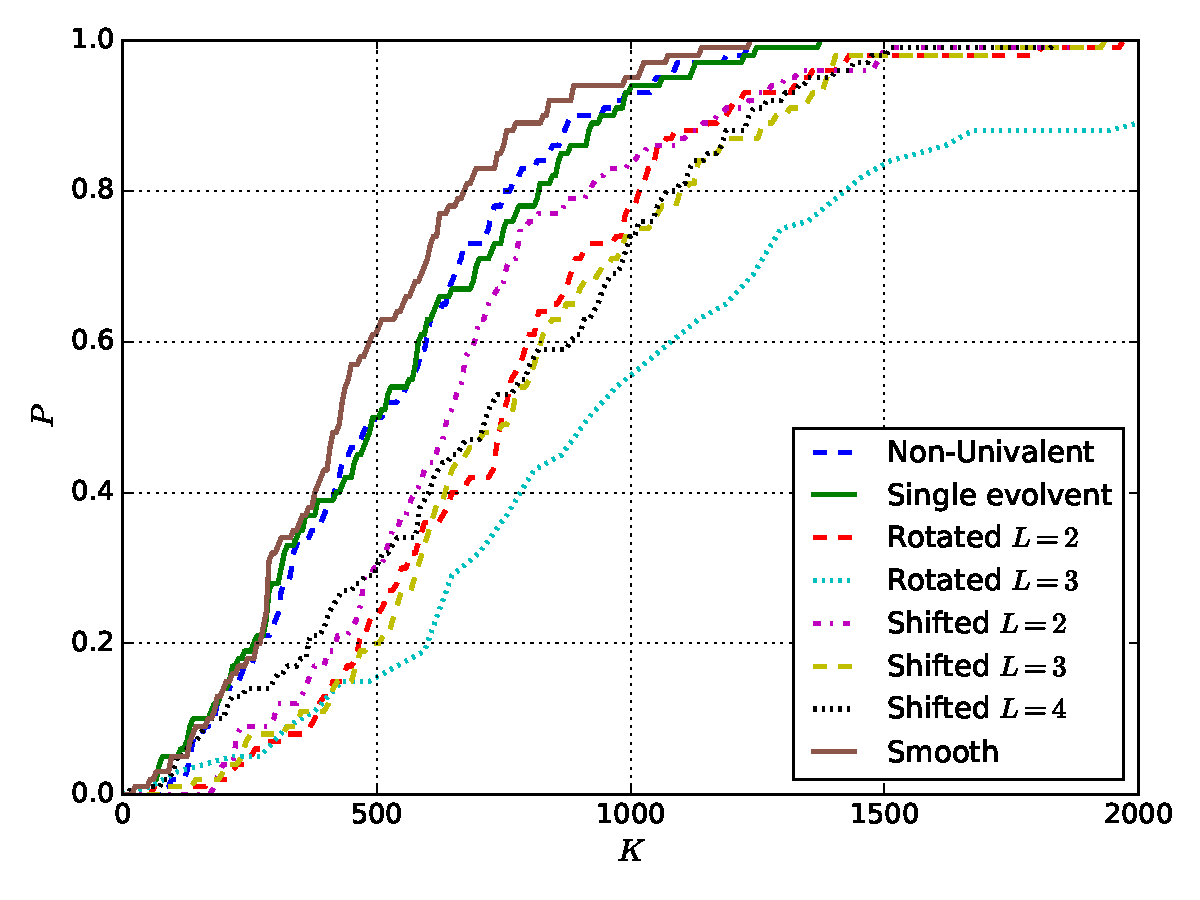
\includegraphics[width=.5\textwidth]{pictures/gklsS2d_same_r_opt_pt_op.pdf}}\label{fig:gkls2d_acc}}
    \subfloat[Minimal $r$]{{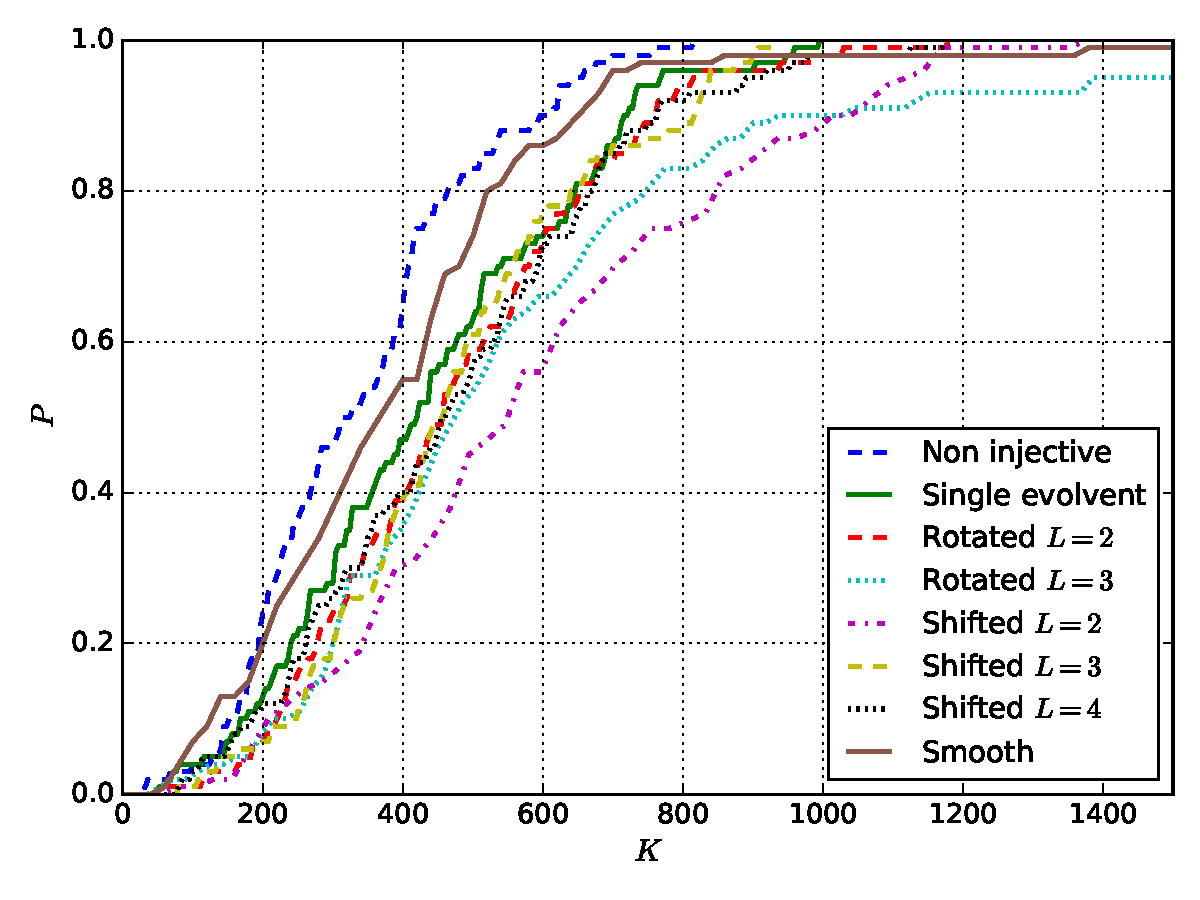
\includegraphics[width=.5\textwidth]{pictures/gklsS2d_opt_pt_op.pdf}}\label{fig:gkls2d_opt}}
    \caption{Operating characteristics on GKLS 2d Simple class}
\end{figure}

На классе GKLS 2d Simple при минимальном \(r\) неинъективная и множественные развёртки имеют значительное преимущество над единственной развёрткой (рис. \ref{fig:gkls3d_opt}). Значение \(r=4.5\) является завышенным для вращаемой и сдвиговой развёрток (рис. \ref{fig:gkls3d_acc}).

\begin{figure}[ht]
    \centering
    \subfloat[$r=4.5$]{{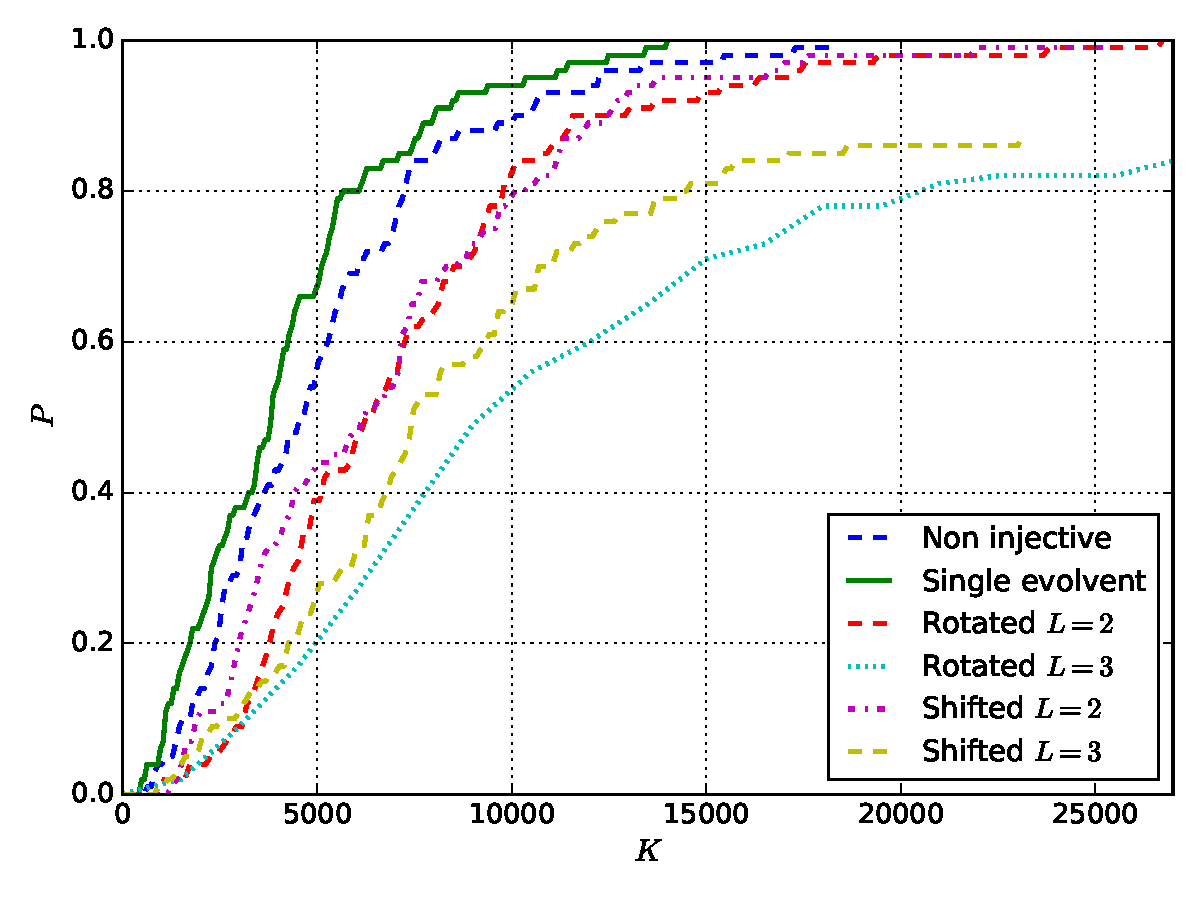
\includegraphics[width=.5\textwidth]{pictures/gklsS3d_same_r_opt_pt_op.pdf}}\label{fig:gkls3d_acc}}
    \subfloat[Minimal $r$]{{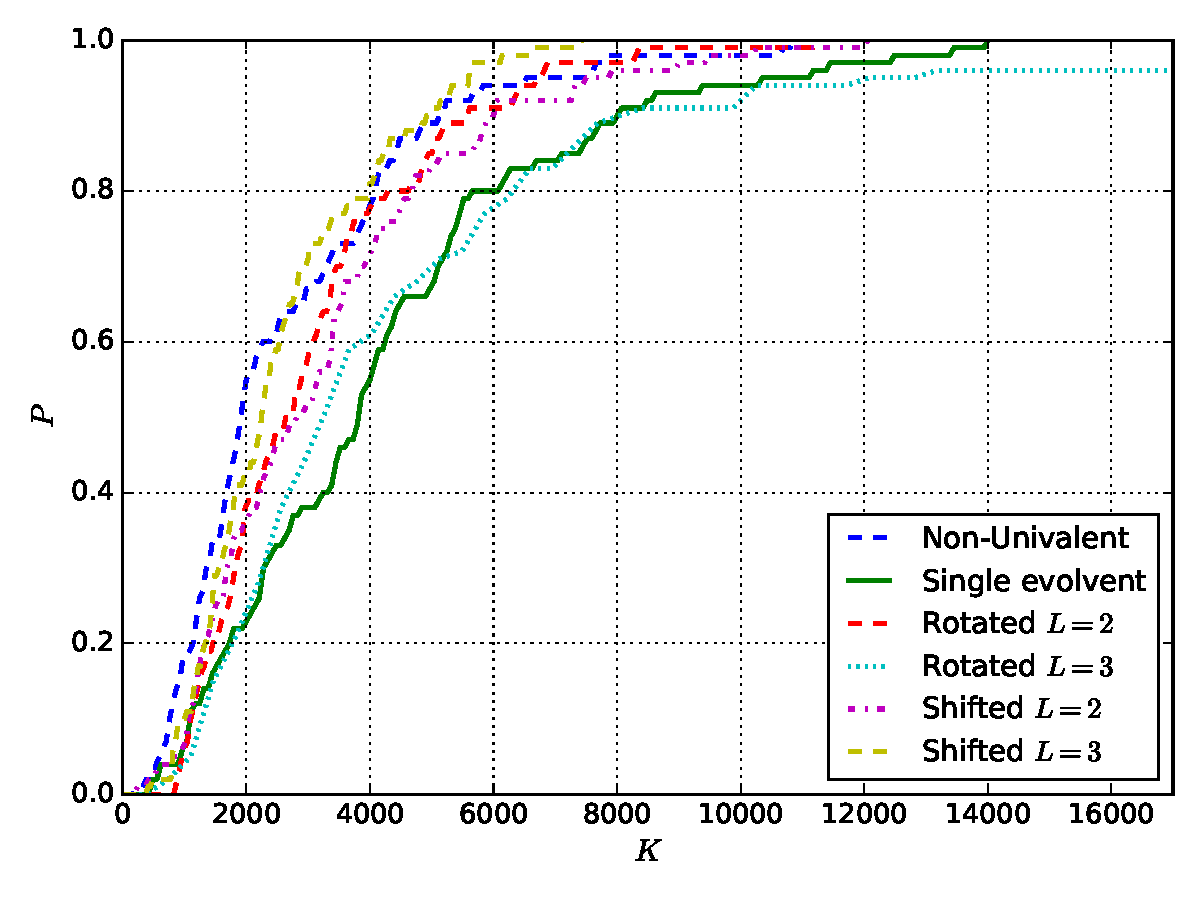
\includegraphics[width=.5\textwidth]{pictures/gklsS3d_opt_pt_op.pdf}}\label{fig:gkls3d_opt}}
    \caption{Operating characteristics on GKLS 3d Simple class}
\end{figure}

\paragraph{Накладные расходы при использовании сдвиговой развёртки.}
Во всех представленных выше экспериментах при построении операционной характеристики учитывалось количество вычислений целевой функции из класса GKLS, однако в случае сдвиговой развёртки индексный метод решает задачу с ограничением \(g_0\) из (\ref{6_g0}). В точках, где \(g_0\) нарушено, значение целевой функции не вычисляется. Эти точки, тем не менее, хранятся в поисковой информации, создавая дополнительные расходы вычислительных ресурсов. В таблице \ref{tab:shifted_g0} приведено среднее количество обращение к \(g_0\) и целевой функции. При \(L=3\) ограниение \(g_0\) вычисляется почти в 20 раз чаще, чем целевая функция \(\varphi\), т. е. \(95\%\) всей поисковой информации приходится на вспомогательные точки. Такие накладные расходы приемлемы при решении задач малой размерности с трудоёмкими целевыми функциями, но при росте размерности и общего количества испытаний выгоднее использовать другие типы развёрток.

\begin{table}
\begin{center}
\caption{Среднее количество вычислений \(g_0\) и \(\varphi\) при решении задач класса GKLS 3d Simple с помощью сдвиговой развёртки}
  \begin{tabular}{|l|{c}|{c}|{c}|}
    \hline
  $L$ & $calc(g_0)$ & $calc(\varphi)$ & $\frac{calc(g_0)}{calc(\varphi)}$ ratio \\
  \hline
  2 & 96247.9  & 6840.14 & 14.07\\
  \hline
  3 & 153131.0 & 7702.82 & 19.88\\
  \hline
  \end{tabular}
  \label{tab:shifted_g0}
\end{center}
\end{table}

%------------------------------------------------------------------------------
\subsection{Параллельные вращаемые развертки}
\label{sec:results_parallel}
Чтобы оценить эффективность параллельного алгортима из секции \ref{sec:parallel_evolvents} были проведены вычислительные эксперименты на классах GKLS 4d (Hard, Simple) и GKLS 5d (Hard, Simple). Значения \(r\) во всех экспериментах равно 5.0, размер \(\delta\)-окрестности известного решения увеличен до 0.3. При решении серий задач использовалось до 8 узлов кластера и до 32 вычислительных потоков на каждом узле.

В таблице \ref{tab:iterations} приведено среднее количество итераций при решении 100 задач из каждого из рассматриваемых классов. При увеличении числа узлов и числа потоков на каждом узле количество итераций заметно сокращается (за исключением класса GKLS 4d Simple при переходе с 1 узла на 4 узла в однопоточном режиме).

\begin{table}
  \centering
  \caption{Averaged numbers of iterations executed by the parallel algorithm for solving the test optimization problems}
  \label{tab:iterations}
  \begin{tabular}{cccccccc}
    \cline{3-8}\noalign{\smallskip}
    \multicolumn{2}{c}{  } & \textit{p} & \multicolumn{2}{c}{$N=4$} & & \multicolumn{2}{c}{$N=5$}   \\
    \noalign{\smallskip} \cline{4-5} \cline{7-8}  \noalign{\smallskip}
    \multicolumn{2}{c}{  } & & \textit{Simple} & \textit{Hard} & & \textit{Simple} & \textit{Hard}  \\
    \noalign{\smallskip}\hline
    I &
    \parbox{0.25\textwidth}{
    \begin{center}
    \textbf{1 cluster node}
    \end{center}		}
      & \textit{1} & 12167 & 25635 & & 20979 & 187353  \\
    &  & \textit{32} & 328 & 1268  & &   898 & 12208 \\
    \hline \noalign{\smallskip}
II  & \textbf{4 cluster nodes}  %\multirow{3}{*}{}
  & \textit{1} & 25312 & 11103 & & 1472 & 17009 \\
&   & \textit{32} & 64 &   913 & & 47 & 345 \\
    \noalign{\smallskip}\hline	\noalign{\smallskip}
III & \textbf{8 cluster nodes} %\multirow{3}{*}{}
  & \textit{1}  & 810 & 4351 & & 868 & 5697  \\
& & \textit{32} & 34  & 112  & & 35  & 868 \\
    \noalign{\smallskip}\hline
  \end{tabular}
\end{table}

Если считать, что затраты на параллелизм пренебрежимо малы по сравнению с затратами на вычисление целевых функций в задачах оптимизации, то ускорение по времени от использования параллельного метода будет равно ускорению по итерациям. Однако, в действительности это предположение не всегда справедливо. Во всех численных экспериментах время вычисления целевой функции занимает примерно $10^{-3}$с. В таблице \ref{tab:speedup} приведено ускорение по итерациям и в куглых скобках ускорение по времени. В первой строке таблицы, соответствующей последовательному режиму, в скобках приведено среднее время решения одной задачи. Из таблицы видно, что для класов GKLS 4d выгоднее использовать один узел в многопоточном режиме, тогда как для решения более сложных пятимерных задач лучше использовать несколько узлов, каждый из которых работает в параллельном режиме.

\begin{table}
  \centering
  \caption{Speedup of parallel computations executed by the parallel algorithm}
  \label{tab:speedup}
  \begin{tabular}{cccccccc}
    \cline{3-8}\noalign{\smallskip}
    \multicolumn{2}{c}{  } & \textit{p} & \multicolumn{2}{c}{$N=4$} & & \multicolumn{2}{c}{$N=5$}   \\
    \noalign{\smallskip} \cline{4-5} \cline{7-8}  \noalign{\smallskip}
    \multicolumn{2}{c}{  } & & \textit{Simple} & \textit{Hard} & & \textit{Simple} & \textit{Hard}  \\
    \noalign{\smallskip}\hline
    I &
    \parbox{0.25\textwidth}{
    \begin{center}
    \textbf{1 cluster node}
    \end{center}		}
    & \textit{1}   & 12167(10.58s) & 25635(22.26s) & & 20979(22.78s) & 187353(205.83s)  \\
  &  & \textit{32} & 37.1(18.03) & 20.2(8.55)  & &  23.3(8.77) & 15.4(9.68) \\
  \hline \noalign{\smallskip}
II  & \textbf{4 cluster nodes}  %\multirow{3}{*}{}
& \textit{1} &        0.5(0.33) & 2.3(0.86)  & & 14.3(6.61) & 11.0(6.06) \\
&   & \textit{32} & 190.1(9.59) & 28.1(1.08) & & 446.4(19.79) & 543.0(43.60) \\
  \noalign{\smallskip}\hline	\noalign{\smallskip}
III & \textbf{8 cluster nodes} %\multirow{3}{*}{}
& \textit{1}    & 15.0(6.05)  & 5.9(2.36)   & & 24.2(17.56)  & 32.9(24.87)  \\
& & \textit{32} & 357.9(2.36) & 228.9(2.64) & & 582.8(20.96) & 793.0(33.89) \\
    \noalign{\smallskip}\hline
  \end{tabular}
\end{table}

%------------------------------------------------------------------------------
\section{Conclusions}
В работе рассмотрены 5 различных отображений типа кривой Пеано, применяемых для редукции размерности в задачах глобальной оптимизации.
Из предварительного сравнения, проведенного в секции \ref{sec:seq_comp}, можно сделать слудующие выводы:
\begin{itemize}
  \item гладкая и неинъективная развёртки показывают наилучший результат в задачах малой размерности и могут быть успешно применены при решении задач с трудоемкими целевыми функциями. Особенности этих развёрток не позволяют создать на их основе масштабируемый на несколько узлов кластера алгоритм оптимизации.
  \item сдвиговые развёртки привносят большие накладные расходы на работу метода из-за того, что требуется добавления в задачу (\ref{eq:task}) вспомогательного функционального ограничения. Эксперименты показали, что до 95\% поисковой информации приходится на точки, в которых вичисляется только вспомогательное ограничение. Сдвиговые развёртки могут быть использованы в качестве основы для параллельного алгоритма из секции \ref{sec:parallel_evolvents}, однако расходы на обработку дополнительных точек, скорее всего, приведут к малому коэффициенту ускорения от параллельности. Однако, при достаточно трудоёмкой целевой функции их использование может иметь смысл.
  \item вращаемые развёртки обеспечили приемлемую скорость сходимости на задачах малой размерности в последовательном случае. Их использование не приводит к введению дополнительных ограничений, что позволяет построить эффективный параллельный алгоритм на их основе.
\end{itemize}

В секции \ref{sec:results_parallel} приведены результаты численных экспериментов, которые показывают, что алгоритм из раздела \ref{sec:parallel_evolvents} на основе вращаемых развёрток позволяет получить ускорение до 43 раз при решении серии задач с использованием нескольких узлов вычислитеьного кластера. Стоит заметить, что в расматриваемых задачах целевые функции не являются трудоёмкими (среднее время вычисления $10^{-3}$с) и в случае более сложных задач показатели ускорения по времени будут приближаться к ускорению по итерациям.

% ---- Bibliography ----
%
% BibTeX users should specify bibliography style 'splncs04'.
% References will then be sorted and formatted in the correct style.
%
% \bibliographystyle{splncs04}
% \bibliography{mybibliography}
%
\begin{thebibliography}{107}

\bibitem{censorZeniosParGO}% (MR1486040)
\newblock Y. Censor and S. A. Zenios,
\newblock \emph{Parallel Optimization: Theory, Algorithms, and Applications},
\newblock Oxford University Press, 1998.

\bibitem{ciegisHentyParGO} (MR2499546)% [10.1007/978-0-387-09707-7]
\newblock R. \v Ciegis, D. Henty, B. K\aa gstr\"om and J. \v Zilinskas,
\newblock \emph{Parallel Scientific Computing and Optimization: Advances and Applications},
\newblock Springer, 2009.

\bibitem{Famularo1999} %(MR1827451) [10.1016/S0005-1098(99)00058-8]
\newblock D. Famularo, P. Pugliese and Y. D. Sergeyev,
\newblock \emph{\emph{A global optimization technique for checking parametric robustness}},
\newblock \emph{Automatica}, \textbf{35} (1999), 1605--1611.

\bibitem{fasanoPinter2013}% (MR3013800) [10.1007/978-1-4614-4469-5]
\newblock G. Fasano and J. D. Pint\'er,
\newblock \emph{Modeling and Optimization in Space Engineering},
\newblock Springer, 2013.

\bibitem{floudasPardalosGOState} %(MR1390521) [10.1007/978-1-4613-3437-8]
\newblock C. A. Floudas and M. P. Pardalos,
\newblock \emph{State of the Art in Global Optimization: Computational Methods and Applications},
\newblock Kluwer Academic Publishers, Dordrecht, 1996.

\bibitem{floudasPardGO}% (MR1147432) [10.1007/s10898-008-9332-8]
\newblock C. A. Floudas and M. P. Pardalos,
\newblock \emph{Recent Advances in Global Optimization},
\newblock Princeton University Press, 2016.

\bibitem{Gablonsky} %(MR1856800) [10.1023/A:1017930332101]
\newblock J. M. Gablonsky and C. T. Kelley,
\newblock \emph{\emph{A locally-biased form of the DIRECT algorithm}},
\newblock \emph{J. Glob. Optim.}, \textbf{21} (2001), 27--37.

\bibitem{horstTuyGO}% (MR1102239) [10.1007/978-3-662-03199-5]
\newblock R. Horst and H. Tuy,
\newblock \emph{Global Optimization: Deterministic Approaches},
\newblock Springer-Verlag, Berlin, 1990.

\bibitem{Kvasov2015}% (MR3585540) [10.1016/j.advengsoft.2014.09.014]
\newblock D. E. Kvasov and Y. D. Sergeyev,
\newblock \emph{\emph{Deterministic approaches for solving practical black-box global optimization problems}},
\newblock \emph{Adv. Eng. Softw.}, \textbf{80} (2015), 58--66.

\bibitem{Menniti}% [10.1016/j.epsr.2007.10.009]
\newblock D. E. Kvasov, D. Menniti, A. Pinnarelli, Y. D. Sergeyev and N. Sorrentino,
\newblock \emph{\emph{Tuning fuzzy power-system stabilizers in multi-machine systems by global optimization algorithms based on
 efficient domain partitions}},
\newblock \emph{Electric Power Systems Research}, \textbf{78} (2008), 1217--1229.

\bibitem{locatelliSchoenGO}% (MR3136805) [10.1137/1.9781611972672]
\newblock M. Locatelli and F. Schoen,
\newblock \emph{Global Optimization: Theory, Algorithms and Applications},
\newblock SIAM, 2013.

\bibitem{luqueAlbaGA}% (MR2808873) [10.1007/978-3-642-22084-5]
\newblock G. Luque and E. Alba,
\newblock \emph{Parallel Genetic Algorithms. Theory and Real World Applications},
\newblock Springer-Verlag, Berlin, 2011.

\bibitem{pardalosZhigljavskyZilinskas2016}% (MR2361744) [10.1007/978-3-319-29975-4]
\newblock M. P. Pardalos, A. A. Zhigljavsky and J. \v Zilinskas,
\newblock \emph{Advances in Stochastic and Deterministic Global Optimization},
\newblock Springer, 2016.

\bibitem{pinterGO}% (MR1374104) [10.1007/978-1-4757-2502-5]
\newblock J. D. Pint\'er,
\newblock \emph{Global Optimization in Action (Continuous and Lipschitz Optimization: Algorithms, Implementations and Applications)},
\newblock Kluwer Academic Publishers, Dordrecht, 1996.

\bibitem{sergeyevStronginLera2013}% (MR3113120) [10.1007/978-1-4614-8042-6]
\newblock Y. D. Sergeyev, R. G. Strongin and D. Lera,
\newblock \emph{Introduction to Global Optimization Exploiting Space-filling Curves},
\newblock Springer, 2013.

\bibitem{strongin1978}% (MR509033)
\newblock R. G. Strongin,
\newblock \emph{Numerical Methods in Multi-Extremal Problems (Information-Statistical Algorithms)},
\newblock Moscow: Nauka, In Russian, 1978.

\bibitem{Strongin1992}% (MR1263606) [10.1007/BF00122428]
\newblock R. G. Strongin,
\newblock \emph{\emph{Algorithms for multi-extremal mathematical programming problems employing a set of joint space-filling curves}},
\newblock \emph{J. Glob. Optim.}, \textbf{2} (1992), 357--378.

\bibitem{stronginGergelBarkalovParGO}
\newblock R. G. Strongin, V. P. Gergel, V. A. Grishagin and K. A. Barkalov,
\newblock \emph{Parallel Computations for Global Optimization Problems},
\newblock Moscow State University (In Russian), Moscow, 2013.

\bibitem{strSergGO}5 (MR1797058) [10.1007/978-1-4615-4677-1]
\newblock R. G. Strongin and Y. D. Sergeyev,
\newblock \emph{Global Optimization with Non-convex Constraints. Sequential and Parallel Algorithms},
\newblock Kluwer Academic Publishers, Dordrecht (2000, 2nd ed. 2013, 3rd ed. 2014).

\bibitem{zilinskTornGO}% (MR1100586) [10.1007/3-540-50871-6]
\newblock A. T\"orn and A. \v Zilinskas,
\newblock \emph{Global Optimization},
\newblock Springer, 1989.

\bibitem{zhigljavskyRandGO}% (MR1187048) [10.1007/978-94-011-3436-1]
\newblock A. A. Zhigljavsky,
\newblock \emph{Theory of Global Random Search},
\newblock Kluwer Academic Publishers, Dordrecht, 1991.

\bibitem{Strongin1991}
Strongin, R.G.: Parallel multi-extremal optimization using a set of evolvents. Comp. Math. Math. Phys. \textbf{31(8)}, 37--46 (1991)

\bibitem{Gergel2009}
Strongin, R.G., Gergel, V.P., Barkalov, K.A.: Parallel methods for global optimization problem solving. Journal of instrument engineering. \textbf{52}, 25--33 (2009) (In Russian)

\bibitem{Gaviano2003}
Gaviano, M., Kvasov, D.E, Lera, D., and Sergeyev, Ya.D.: Software for generation of classes of test functions with known local and global minima for global optimization. ACM Transactions on Mathematical Software 29(4), 469--480 (2003)

\bibitem{grishaginClass}
Grishagin, V.A.: Operating Characteristics of Some Global Search Algorithms. Problems of Statistical Optimization 7, 198--206 (1978) (In Russian)

\bibitem{globalizerSystem}
Gergel V.P., Barkalov K.A., and Sysoyev A.V: Globalizer: A novel supercomputer software system for solving time-consuming global optimization problems. Numerical Algebra, Control \& Optimization 8(1), 47--62, 2018

\end{thebibliography}
\end{document}
